\qquad Окрім моделювання ВАХ діодів я також дослідив ВАХ світлодіода, що мав у комплекті з Arduino. Для світлодіода було досить складно отримати ВАХ, що схожа на результати отримані в результаті моделювання, оскільки необхідним був досить малий струм.\\У роботі з Arduino я використовув наступну схему, що дозволяла виміряти напругу на резисторі, визначивши сигнал, що подається на вихід А0, а також визначити напругу на світодіоді, знайшовши різницю між сигналами, що подається на вихід А0 і А1.
\begin{figure}[ht]

\centering

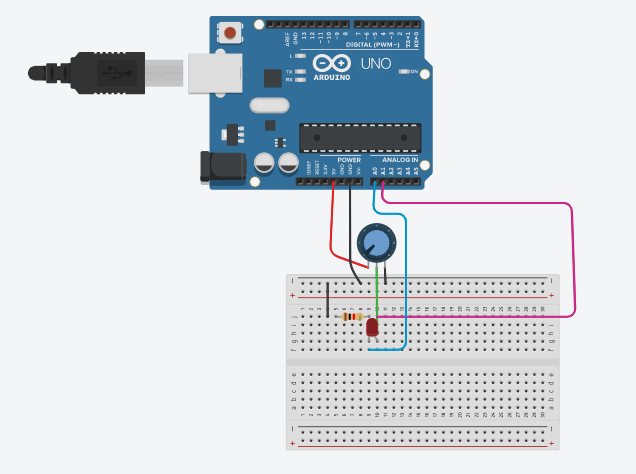
\includegraphics[width=0.6\linewidth]{АрдуиноСхема.png}

\caption{Схема проекту}

\label{ArduinoShema}

\end{figure}

Замість генератору гармонічного сигналу був використаний потенциометр, що дає змогу змінювати напругу на світодіоді від 0 до 5 В.\\ Для ардуіно ми не маємо точних амперметрів та вольтметрів, тому на шкалі X та Y маємо лише відносне значення сили струму та напруги.
\begin{figure}[ht]

\centering

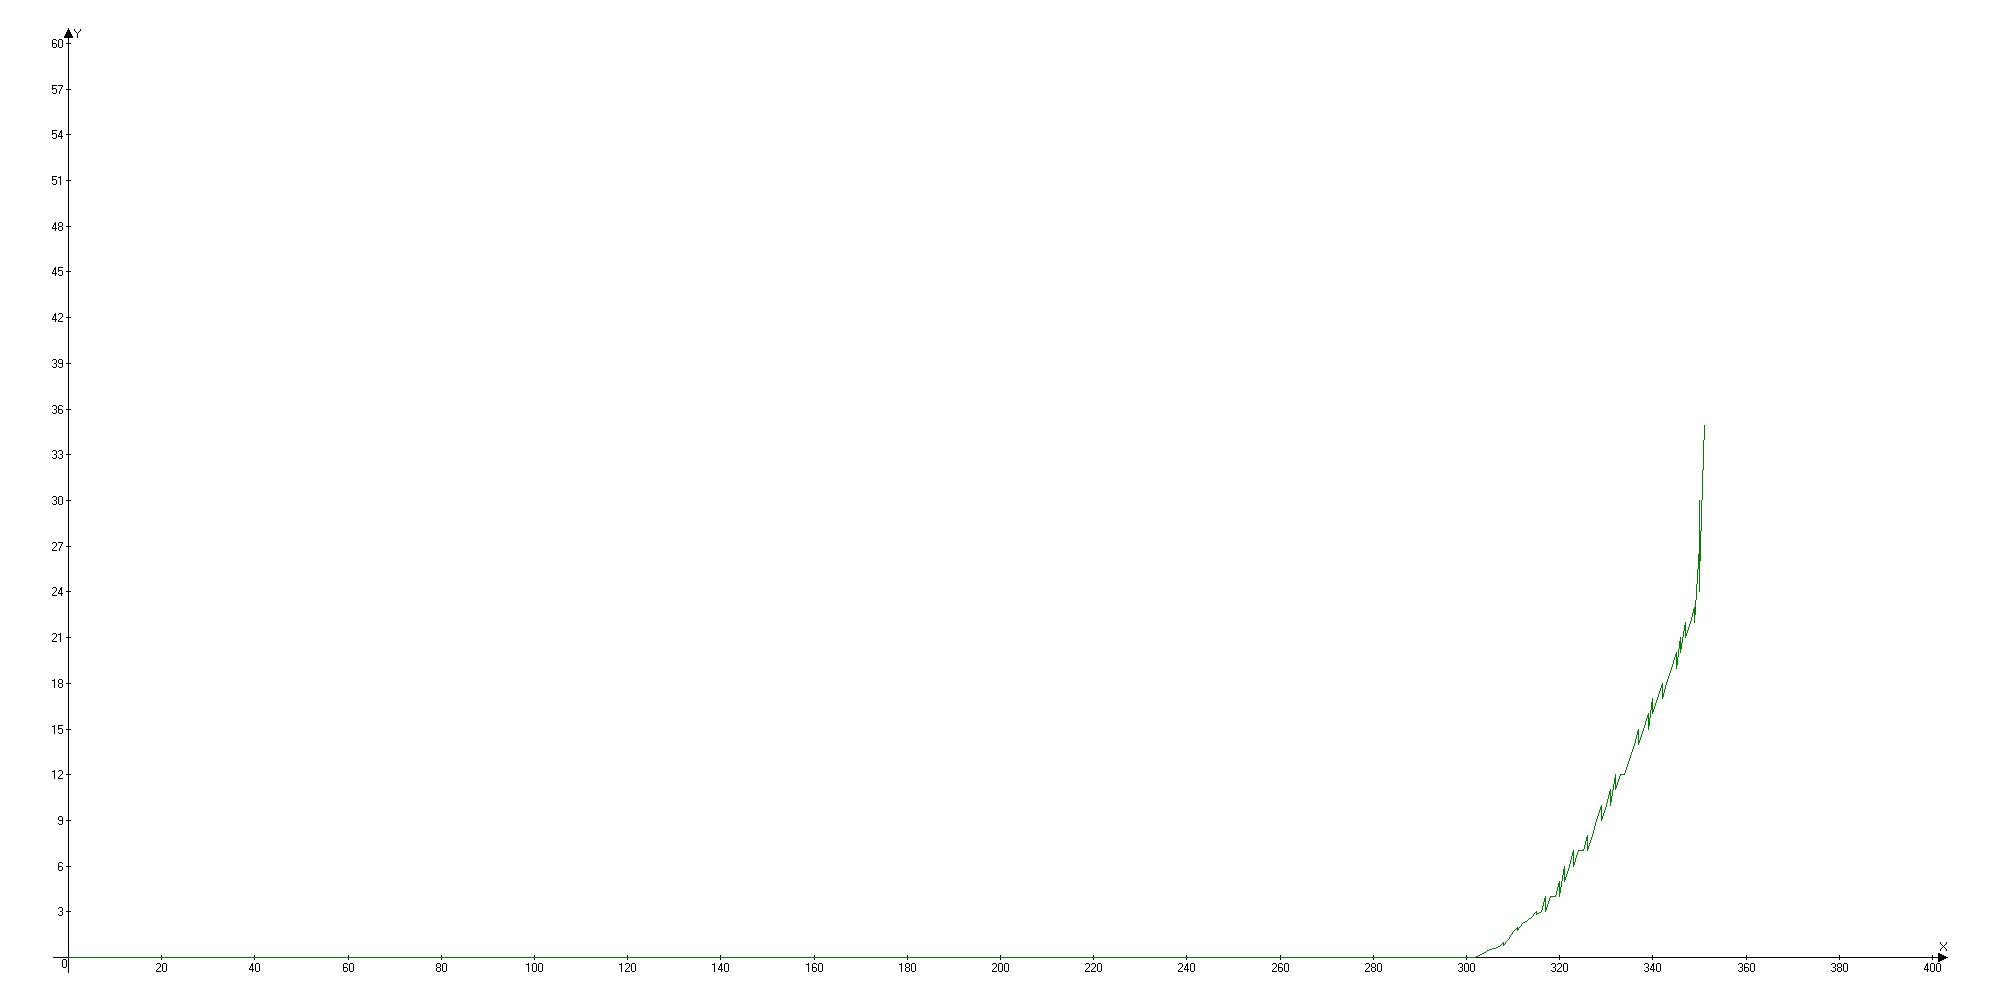
\includegraphics[width=0.8\linewidth]{Ардуино1.png}

\caption{Результати вимірів}

\label{Arduino1Rez}

\end{figure}
